\documentclass[../../../../main.tex]{subfiles}
\begin{document}

\begin{flushright}
\footnotesize\textit{【自動文字起こし・要確認】}
\end{flushright}

\noindent
[\textbf{解}]

\noindent
正 $n$ 角形の一辺の長さを $l_n$ とおくと, $l_n = 2 r \sin \frac{\pi}{n}$ である $\dots$ ①

\begin{center}
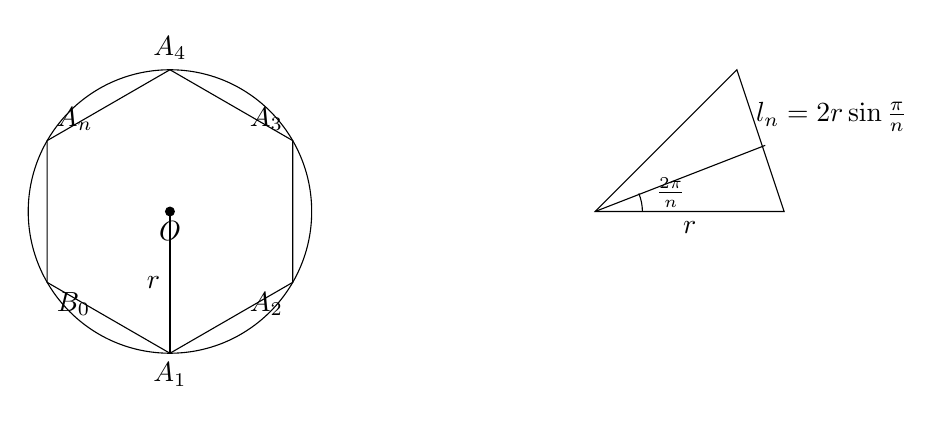
\begin{tikzpicture}[scale=1.2]
    % Left circle and polygon diagram
    \begin{scope}[shift={(0,0)}]
        \draw (0,0) circle (1.5);
        \fill (0,0) circle (1.5pt) node[below]{$O$};
        % Regular polygon vertices
        \foreach \i in {1,...,6} {
            \coordinate (A\i) at ({90 - (\i-1)*60}:1.5);
        }
        \draw (A1) -- (A2) -- (A3) -- (A4) -- (A5) -- (A6) -- cycle;
        \node[above] at (A1) {$A_4$};
        \node[above left] at (A2) {$A_3$};
        \node[below left] at (A3) {$A_2$};
        \node[below] at (A4) {$A_1$};
        \node[below right] at (A5) {$B_0$};
        \node[above right] at (A6) {$A_n$};
        \draw (0,0) -- (A4) node[midway,left]{$r$};
    \end{scope}
    
    % Right sector diagram
    \begin{scope}[shift={(4.5,0)}]
        \draw (0,0) -- (2,0) -- (1.5,1.5) -- cycle;
        \draw (0,0) -- (1.8, 0.7);
        \draw (0.5,0) arc (0:22.5:0.5);
        \node at (0.8,0.2) {\small $\frac{2\pi}{n}$};
        \node[below] at (1,0) {$r$};
        \node[right] at (1.6,1.0) {$l_n = 2r \sin \frac{\pi}{n}$};
    \end{scope}
\end{tikzpicture}
\end{center}

\noindent
題意から扇形 $A_{k+2} A_{k+1} B_k$ ($k \ge 0, B_0 = A_1$) の半径を $r_k$ とすると
\[
\begin{cases}
r_0 = 1 \cdot l_n \\
r_{k+1} = r_k + l_n
\end{cases}
\]
から, 等差数列の公式より, $r_k = (k+1) l_n$ であり, 中心角は $\frac{2\pi}{n}$ だから, 扇形 $A_{k+2} A_{k+1} B_k$ の面積 $T_k$ は
\[
T_k = \frac{1}{2} \cdot \frac{2\pi}{n} \cdot r_k^2 = \frac{\pi}{n} l_n^2 (k+1)^2
\]

\noindent
よって, 扇形の面積の総和 $T$ は
\[
T = \sum_{k=0}^{n-1} \frac{\pi}{n} l_n^2 (k+1)^2
\]
\[
= \sum_{k=1}^n \frac{\pi}{n} l_n^2 k^2
\]
\[
= \frac{1}{6} \pi (n+1)(2n+1) l_n^2 \quad \dots \text{②}
\]

\noindent
一方, 正 $n$ 角形の面積 $S$ は, 右の小三角形の面積の $n$ 倍で,

\begin{minipage}{0.7\textwidth}
\[
\frac{S}{n} = \frac{1}{2} \cdot r^2 \cdot \sin \frac{2\pi}{n}
\]
\[
S = \frac{1}{2} n r^2 \sin \frac{2\pi}{n} \quad \dots \text{③}
\]
\end{minipage}
\begin{minipage}{0.28\textwidth}
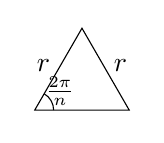
\begin{tikzpicture}[scale=0.8]
    \draw (0,0) -- (1.5,0) -- (0.75, 1.3) -- cycle;
    \draw (0.3,0) arc (0:60:0.3);
    \node at (0.4,0.3) {\small $\frac{2\pi}{n}$};
    \node[left] at (0.4,0.7) {$r$};
    \node[right] at (1.1,0.7) {$r$};
\end{tikzpicture}
\end{minipage}

\vspace{1em}
\noindent
①, ②, ③から
\[
S_n = S + T = \frac{1}{2} n r^2 \sin \frac{2\pi}{n} + \frac{\pi}{6} (n+1)(2n+1) r^2 \cdot 4 \sin^2 \frac{\pi}{n}
\]
\[
= \frac{1}{2} r^2 \cdot \frac{\sin \frac{2\pi}{n}}{\frac{2\pi}{n}} \cdot 2\pi + \frac{2\pi}{3} r^2 \left( \frac{\sin \frac{\pi}{n}}{\frac{\pi}{n}} \right)^2 \pi^2 \left( 1 + \frac{1}{n} \right) \left( 2 + \frac{1}{n} \right)
\]
\[
\to \pi r^2 + \frac{4}{3} \pi^3 r^2 \quad \left( n \to \infty, \text{この時 } \frac{2\pi}{n}, \frac{\pi}{n} \to 0 \right)
\]

\newpage

\end{document}
